% A stub for the re-linking figure.
\begin{figure}
\begin{subfigure}[t]{0.48\textwidth}
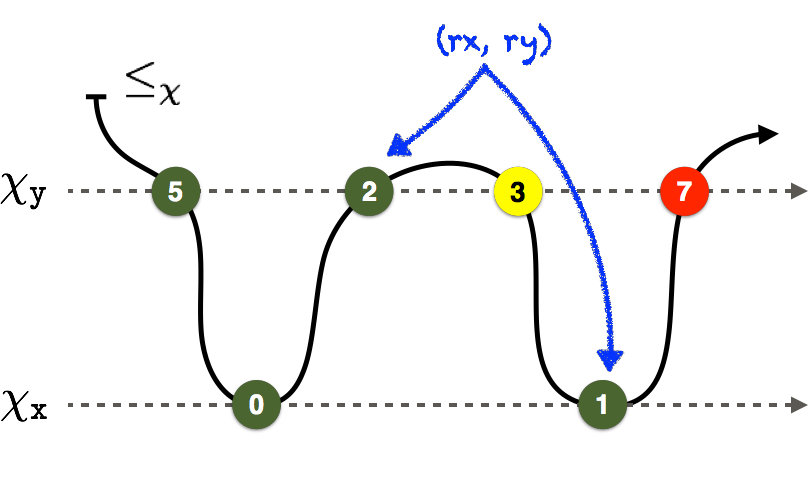
\includegraphics[height=5cm]{res/before-relink-trans}
\caption{\label{fig:relink:before} Before re-link}
\end{subfigure} \hfill
\begin{subfigure}[t]{0.48\textwidth}
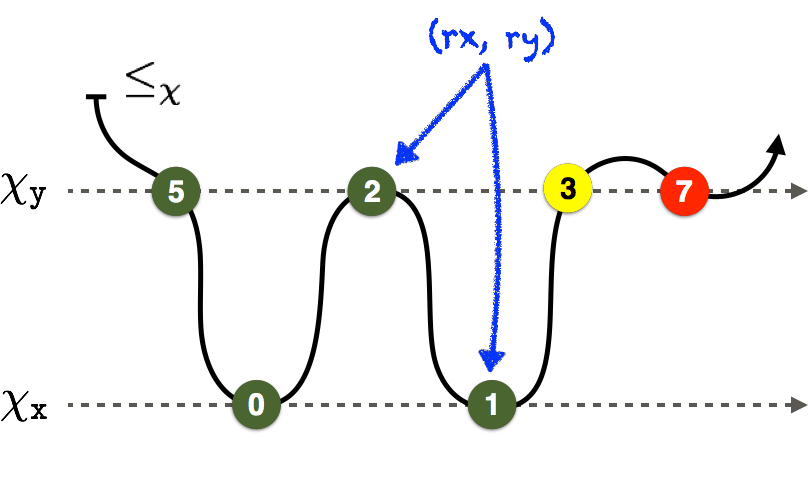
\includegraphics[height=4.5cm]{res/after-relink-trans}
\caption{\label{fig:relink:after} After re-link}
\end{subfigure}%
%
\caption{\label{fig:relink} Atomic re-link: $(rx,ry)$ points to the
  snapshot that will be returned by {\tt scan}}
\end{figure}

%\gad{FIX ME: subfigure (b) is incorrectly drawn! 1 and 3 are swapped
%  in Real Time as well!!!}

%Fix me: The yellow should be painted red after relink, if we decide
%to go for the (green - red) split for t\left t\right after re-link.
%Though, this would not be stable after we release the lock for scan,
%so why bother. Painting the t|left chain green will suffice, as it
%will be stable.

% Fix me: red marbles have different font colors :(
